\documentclass[12pt, a4paper, simple]{eskdtext}

\usepackage{hyperref}
\usepackage{env}
\usepackage{_sty/gpi_lst}
\usepackage{_sty/gpi_toc}
\usepackage{_sty/gpi_t}
\usepackage{_sty/gpi_p}
\usepackage{_sty/gpi_u}

% Код
% \ESKDletter{О}{Л}{Р}
% \def \gpiDocTypeNum {81}
% \def \gpiDocVer {00}
% \def \gpiCode {\ESKDtheLetterI\ESKDtheLetterII\ESKDtheLetterIII.\gpiStudentGroupName\gpiStudentGroupNum.\gpiStudentCard-0\gpiDocNum~\gpiDocTypeNum~\gpiDocVer}

\def \gpiDocTopic {Отчёт лабораторной работы №\gpiDocNum}

% Графа 1 (наименование изделия/документа)
% \ESKDcolumnI {\ESKDfontII \gpiTopic \\ \gpiDocTopic}

% Графа 2 (обозначение документа)
% \ESKDsignature {\gpiCode}

% Графа 9 (наименование или различительный индекс предприятия) задает команда
% \ESKDcolumnIX {\gpiDepartment}

% Графа 11 (фамилии лиц, подписывающих документ) задают команды
% \ESKDcolumnXIfI {\gpiStudentSurname}
% \ESKDcolumnXIfII {\gpiTeacherSurname}
% \ESKDcolumnXIfV {\gpiTeacherSurname}

\begin{document}
    \begin{ESKDtitlePage}
    \ESKDstyle{empty}
    \begin{center}
        \gpiMinEdu \\
        \gpiEdu \\
        \gpiKaf \\
    \end{center}

    \vfill

    \begin{center}
        \gpiTopic
    \end{center}

    \vfill

    \begin{center}
        \textbf{\gpiDocTopic} \\
        ПО ДИСЦИПЛИНЕ \gpiDiscipline \\
    \end{center}

    \vfill

    \begin{flushright}
        \begin{minipage}[t]{7cm}
            Выполнил:\\
            \PageTitleStudentInfo
            \PageTitleDateField
            \hspace{0pt}

            Проверил:\\
            \PageTitleTeacherInfo
            \PageTitleDateField
        \end{minipage}
    \end{flushright}

    \vfill

    \begin{center}
        \PageTitleCity~\ESKDtheYear
    \end{center}
\end{ESKDtitlePage}

    \ESKDstyle{empty}
    \begin{center}
        \textbf{\gpiDocTopic}
    \end{center}

    % = = = = = = = =
    \paragraph{} \textbf{Тема}: <<\gpiTopicRep>>

    \paragraph{} \textbf{Цель}: разработать простейшие приложения для демонстрации распознавания стандартных жестов.

    \paragraph{} \textbf{Что нужно сделать}:

    (Задание 1) Наследовать интерфейс GestureDetector.OnGestureListener.
    Реализовать метод отслеживания появления касания, то есть палец прижат к экрану (onDown).
    Реализовать метод отслеживающий жест смахивания (onFling).
    Реализовать метод отслеживающий прижатие пальца длительное время (onLongPress).
    Реализовать метод отслеживающий жест прокрутки-пролистывания (onScroll).
    Реализовать метод отслеживающий событие касания и больше никаких событий не происходит короткое время (onShowPress).
    Реализовать метод отслеживающий одиночное нажатие-клик (onSingleTapUp).
    
    Наследовать интерфейс GestureDetector.OnDoubleTapListener.
    Реализовать метод отслеживающий двойное нажатие (onDoubleTap).
    Реализовать метод отслеживающий появление события во время выполнения жеста двойного нажатия,
    включая касание, перемещение, подъема пальца (onDoubleTapEvent).
    Реализовать метод отслеживающий одиночное нажатие-клик (onSingleTapConfirmed).
    
    (Задание 2) Использовать экземпляр класса GestureDetectorCompat, для того, чтобы не переопределять все методы интерфейса,
    а реализовать один, который нам нужен. Реализовать метод отслеживающий жест смахивания (onFling).

    \paragraph{} \textbf{Разработка дизайна}:

    \begin{longtable}{|p{9cm}|p{8cm}|}
        \caption{Скриншоты жестов}
        % \label{tabl:install_virtual_box}
        \endfirsthead
    
        % Заголовок продолжения таблицы на новой странице
        \multicolumn{2}{c}{\tablename\ \thetable\ -- Продолжение таблицы} \\
        \hline
        
        % Заголовок на странице продолжения
        % \textbf{First entry} & \textbf{Second entry} \\
        \multicolumn{1}{|p{9cm}|}{\centering \textbf{Картинка}} & \multicolumn{1}{p{8cm}|}{\centering\textbf{Описание}} \\ \hline
        \endhead
    
        % Если таблица не закончена, то сообщить
        % \hline \multicolumn{2}{r}{\textit{Continued on next page}} \\
        \endfoot
    
        % Заголовок
        \hline
        \multicolumn{1}{|p{9cm}|}{\centering \textbf{Картинка}} & \multicolumn{1}{p{8cm}|}{\centering\textbf{Описание}} \\ \hline
            
        % Элементы
        \raisebox{-\totalheight}{
            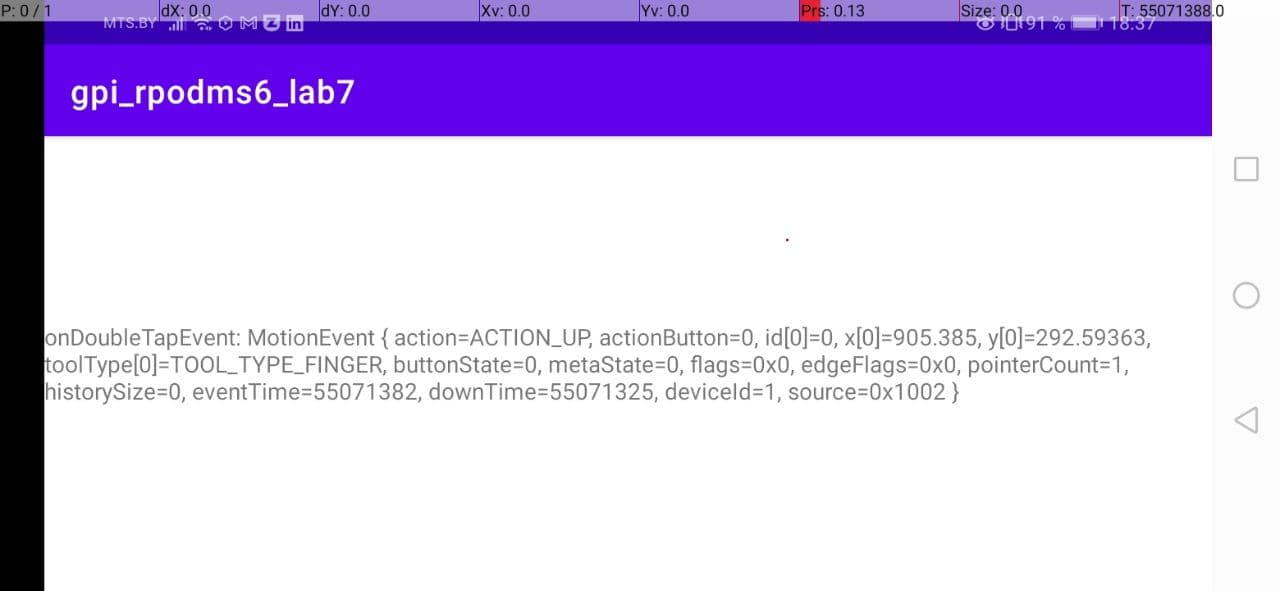
\includegraphics[width=\linewidth]{_assets/onDoubleTapEvent.jpg}
        }
        & onDoubleTapEvent - отслеживает появление события во время выполнения жеста двойного нажатия,
        включая касание, перемещение, подъем пальца. \\ \hline
    
        \raisebox{-\totalheight}{
            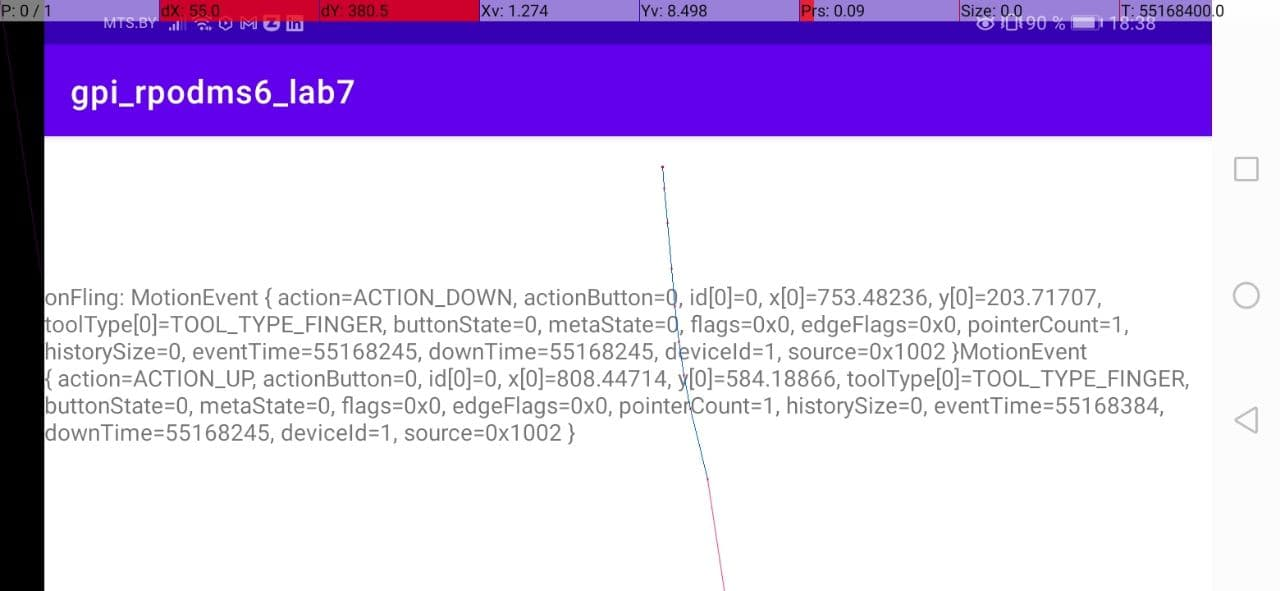
\includegraphics[width=\linewidth]{_assets/onFling.jpg}
        }
        & onFling - отслеживает появление жеста смахивания \\ \hline
    
        \raisebox{-\totalheight}{
            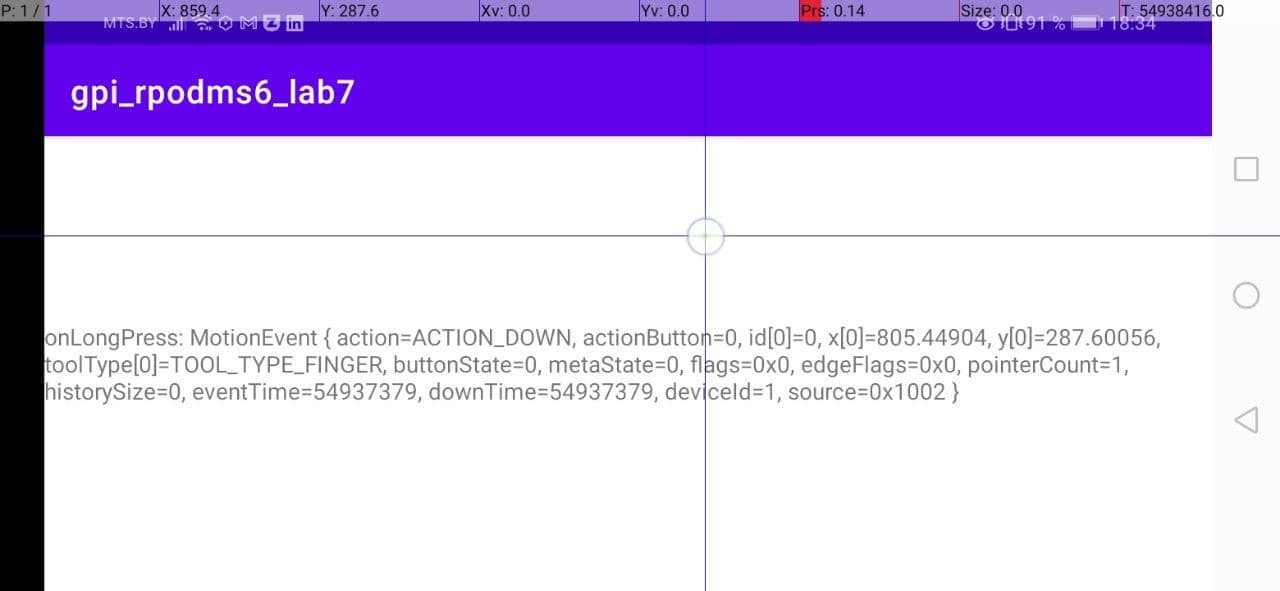
\includegraphics[width=\linewidth]{_assets/onLongPress.jpg}
        }
        & onLongPress - отслеживает удерживание пальца прижатым к экрану длительное время \\ \hline
    
        \raisebox{-\totalheight}{
            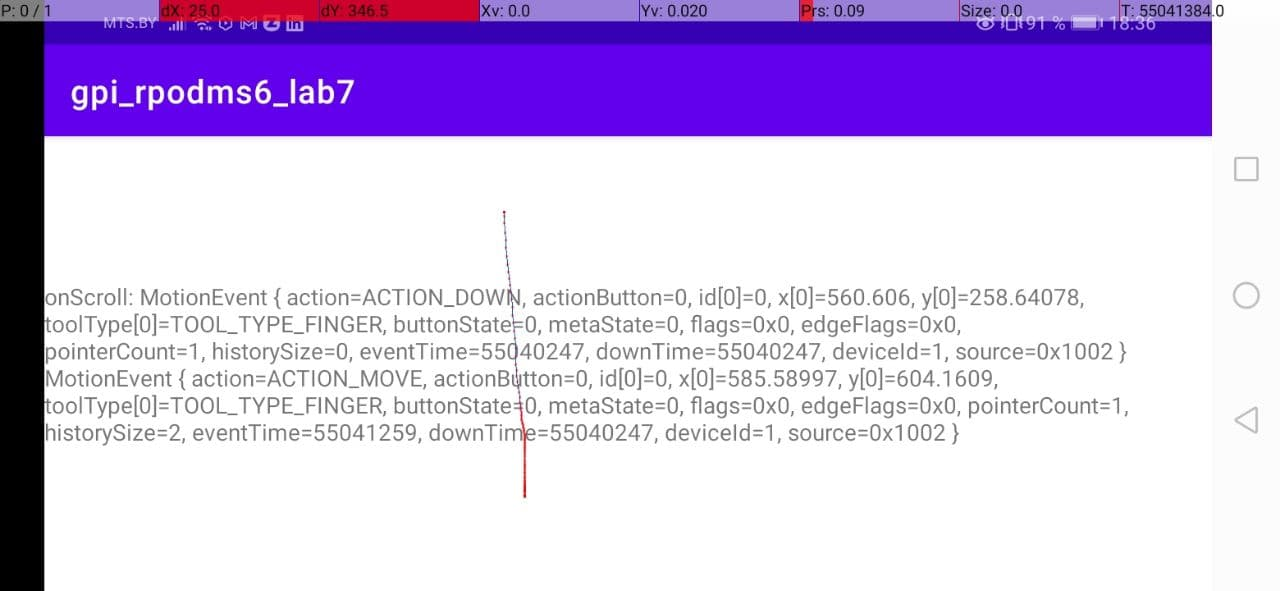
\includegraphics[width=\linewidth]{_assets/onScroll.jpg}
        }
        & onScroll - отслеживает появление жеста прокрутки (пролистывания) \\ \hline
    
        \raisebox{-\totalheight}{
            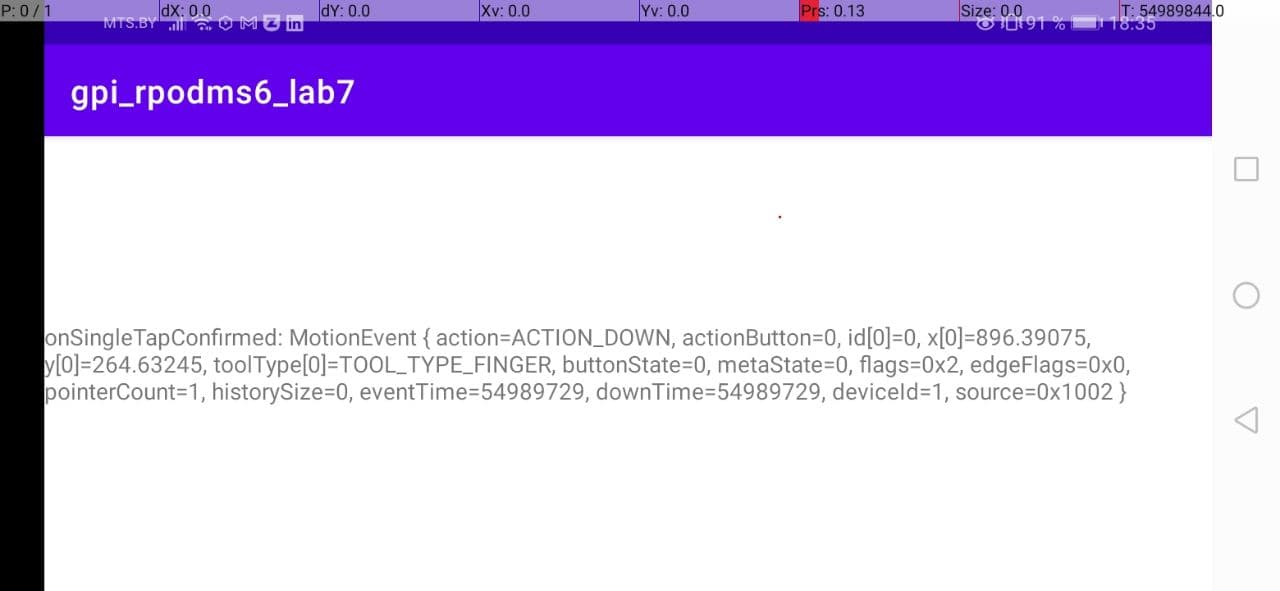
\includegraphics[width=\linewidth]{_assets/onSingleTapConfirmed.jpg}
        }
        & onSingleTapConfirmed - отслеживает появление жеста одиночного нажатия (клик) \\ \hline
    \end{longtable}
    
    \paragraph{} \textbf{Исходный код}: 

    \lstinputlisting[language=java, name=app/src/main/java/.../MainActivity.java]
        {../gpi_src/gpi_rpodms6_lab7/app/src/main/java/io/github/Pavel_Innokentevich_Galanin/gpi_rpodms6_lab7/MainActivity.java}

    \lstinputlisting[language=xml, name=app/src/main/res/layout/activity_main.xml]
        {../gpi_src/gpi_rpodms6_lab7/app/src/main/res/layout/activity_main.xml}

    \lstinputlisting[language=xml, name=app/src/main/res/values/strings.xml]
        {../gpi_src/gpi_rpodms6_lab7/app/src/main/res/values/strings.xml}

    \newpage

    \paragraph{} \textbf{Разработка дизайна}:

    \begin{figure}[h!]
        \centering
        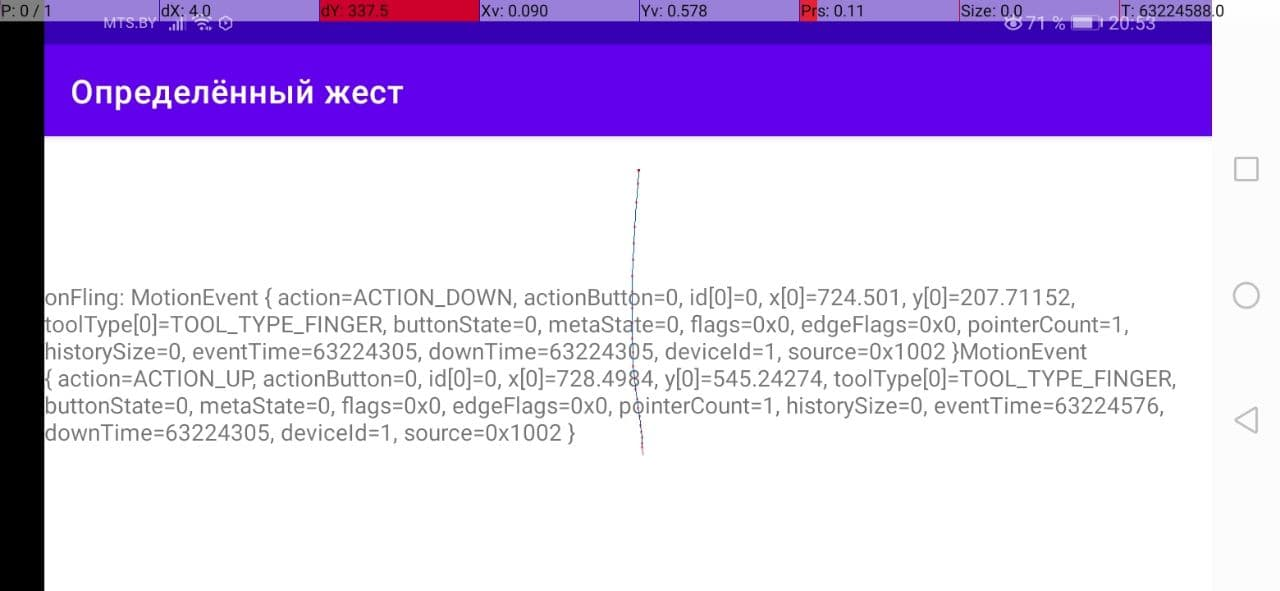
\includegraphics[width=12cm]
            {_assets/GestSubset__onFling.jpg}
        \caption{onFling}
    \end{figure}
 
    \paragraph{} \textbf{Исходный код}: 

    \lstinputlisting[language=java, name=app/src/main/java/.../MainActivity.java]
        {../gpi_src/gpi_rpodms6_lab7__gestsubset/app/src/main/java/io/github/Pavel_Innokentevich_Galanin/gpi_rpodms6_lab7__gestsubset/MainActivity.java}

    \lstinputlisting[language=xml, name=app/src/main/res/layout/activity_main.xml]
        {../gpi_src/gpi_rpodms6_lab7__gestsubset/app/src/main/res/layout/activity_main.xml}

    \lstinputlisting[language=xml, name=app/src/main/res/values/strings.xml]
        {../gpi_src/gpi_rpodms6_lab7__gestsubset/app/src/main/res/values/strings.xml}

    \paragraph{} \textbf{Вывод}:
    
    (1) Наследовал интерфейс GestureDetector.OnGestureListener.\\
    Реализовать методы onDown, onFling, onLongPress, onScroll, onShowPress, onSingleTapUp.
    
    Наследовал интерфейс GestureDetector.OnDoubleTapListener.\\
    Реализовать методы onDoubleTap, onDoubleTapEvent, onSingleTapConfirmed.

    (2) Реализовали экземпляр класса GestureDetectorCompat, для того, чтобы не определять все методы жестов,
    а задать свой определённый жест. Определили метод отслеживания жеста смахивания (onFling). 

    % = = = = = = = =
    \paragraph{} \textbf{Список использованных источников} 
    % \addcontentsline{toc}{section}{СПИСОК ИСПОЛЬЗОВАННЫХ ИСТОЧНИКОВ}
    % \section*{Список использованных источников}
    \begin{enumerate}
        \item[1.] Кондратюк, А.П. Разработка приложений для мобильных операционных систем «Android» :
        ЭУМК для студ. второй ступени (магистратуры) специальности 1-31 81 06 <<Веб-программирование и интернет-технологии>>
        физ.-мат. фак. / А.П. Кондратюк ; Брест. гос. ун-т им. А.С. Пушкина, каф. ПМиИ. – Брест :
        электрон. издание БрГУ, 2016. – 469 с.\\
        §22. Лабораторная работа №4, cc. 389-400.
    \end{enumerate}
    \newpage
\end{document}
